\documentclass[12pt,a4paper]{article}
 
%encoding
%--------------------------------------
\usepackage[utf8]{inputenc}
\usepackage[T1]{fontenc}
%--------------------------------------
 
%Portuguese-specific commands
%--------------------------------------
\usepackage[portuguese]{babel}
%--------------------------------------
 
%Hyphenation rules
%--------------------------------------
\usepackage{hyphenat}
\hyphenation{mate-mática recu-perar}
%--------------------------------------

\usepackage{graphicx}
\graphicspath{ {images/} }
\usepackage{caption}
\usepackage{subcaption}
\usepackage{amsmath}

\begin{document}

\begin{titlepage}

\newcommand{\HRule}{\rule{\linewidth}{0.5mm}} % Defines a new command for the horizontal lines, change thickness here

\center % Center everything on the page
 
%----------------------------------------------------------------------------------------
%	HEADING SECTIONS
%----------------------------------------------------------------------------------------

\textsc{\LARGE INSTITUTO SUPERIOR DE \\[0.2cm] ENGENHARIA DE LISBOA}\\[0.5cm]
\textsc{\LARGE ADEETC  }\\[0.3cm]
\textsc{\Large Licenciatura em Engenharia Informática e Multimédia }\\[0.3cm]
\textsc{\Large Semestre de Verão}\\[0.5cm]
\textsc{\Large 4º Trabalho Prático}\\[0.5cm]

%----------------------------------------------------------------------------------------
%	TITLE SECTION
%----------------------------------------------------------------------------------------

\HRule \\[0.4cm]
{ \huge \bfseries Codificação de Sinais Multimédia}\\[0.03cm] % Title of your document
\HRule \\[1.5cm]

%----------------------------------------------------------------------------------------
%	AUTHOR SECTION
%----------------------------------------------------------------------------------------
\Large \emph{Realizado por:}\\
João \textsc{Santos} nº 39348\\ 
Rui \textsc{Santos} nº 39286\\[2cm] 
%----------------------------------------------------------------------------------------
%	DATE SECTION
%----------------------------------------------------------------------------------------

{\large Junho, 2017}\\[1cm]

%----------------------------------------------------------------------------------------
%	LOGO SECTION
%----------------------------------------------------------------------------------------


\includegraphics[scale=0.3]{iselLogo.jpg}\\[1cm]
 
%----------------------------------------------------------------------------------------
\vfill % Fill the rest of the page with whitespace
\end{titlepage}

%-------------------------------------------------------
\tableofcontents
\newpage
\listoffigures
%\listoftables
\newpage
%-------------------------------------------------------
\section{Introdução}
O quarto trabalho prático da disciplina de Codificação de Sinais Multimédia tem como objetivo o estudo e a implementação dos princípios  básicos da codificação de vídeo. Através de um conjunto de frames disponibilizados, vão ser implementadas três formas distintas de codificação de vídeo, das quais:
\begin{enumerate}
  \item Codificação de cada frame da sequência de vídeo utilizando um codificador JPEG, como o desenvolvido no trabalho 3, considerando que cada frame é uma intra-frame (I).
  \item No segundo ponto é considerado que todas as frames são inter-frames (P) à exceção da primeira que é uma intra-frame (I). As inter-frames (P) são obtidas através da diferença entre a frame a codificar e a intra-frame (I). O ponto 2 é implementado \textbf{sem} compensação de movimento. 
  \item Tal como no ponto 2, é considerado que as frames são inter-frames (P) à exceção da primeira que é uma intra-frame (I). Neste ponto do trabalho é realizada a predição da frame a codificar com base na I-frame \textbf{com} compensação de movimento.
  \end{enumerate} 
  
Com os três tipos de codificação referidos em cima implementados foram desenvolvidos métodos que permitem calcular os valores da Taxa de Compressão, relação sinal-ruído, entropia da frame a transmitir, energia média por píxel e o tempo de compressão e descompressão de cada ponto referido em cima. Posteriormente vão ser apresentados os resultados obtidos em forma da tabelas e gráficos para cada um dos resultados.
\newpage
\section{Desenvolvimento}
\subsection{Codificação considerando cada frame como uma intra-frame}
O primeiro método de codificação desenvolvido no trabalho requer uma codificação considerando cada frame como uma intra-frame (I). Neste caso, cada frame da sequência de vídeo é codificada sem qualquer relação com as frames anteriores. Para tal, foi utilizado o codificador JPEG disponibilizado na biblioteca do OpenCV. Ou seja, para cada frame da sequência de vídeo disponibilizada foi aplicado o seguinte método:\\
\newline
cv2.imwrite("frame\_x.jpeg",img\_x,(cv2.IMWRITE\_JPEG\_QUALITY,qualidade))
\newline

Esta função recebe como argumentos o \textit{pathname} de cada frame, o \textit{array} da frame em questão e realiza a codificação baseada num fator de qualidade introduzido por nós. É possível observar nas Figuras 1 e 2 a codificação realizada para dois fatores de qualidade distintos, respetivamente, 10 e 75\%. 

\begin{figure}[h]
	\centering
    \begin{minipage}{0.45\textwidth}
        \centering
        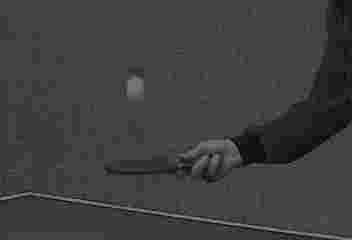
\includegraphics[width=0.9\textwidth]{imagens/10_bola_1.jpeg}
        \caption{Frame 1 codificada com uma qualidade de 10\%.}
    \end{minipage}\hfill
    \begin{minipage}{0.45\textwidth}
        \centering
        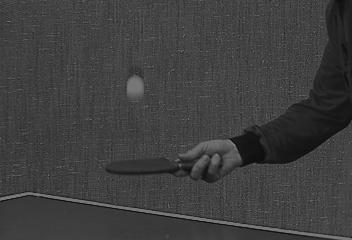
\includegraphics[width=0.9\textwidth]{imagens/75_bola_1.jpeg}
        \caption{Frame 1 codificada com uma qualidade de 75\%.}
    \end{minipage}
\end{figure}

Seguidamente foram realizado os cálculos das Taxas de Compressão, Relação Sinal-Ruído, Entropia e Energia média por píxel. Sendo os resultados obtidos apresentados nas Figuras 3, 4, 5 e 6, para motivos de simplificação os dados apresentados nos gráficos são referentes apenas a um fator de qualidade de 75\%.
\begin{figure}[h]
	\centering
    \begin{minipage}{0.45\textwidth}
        \centering
        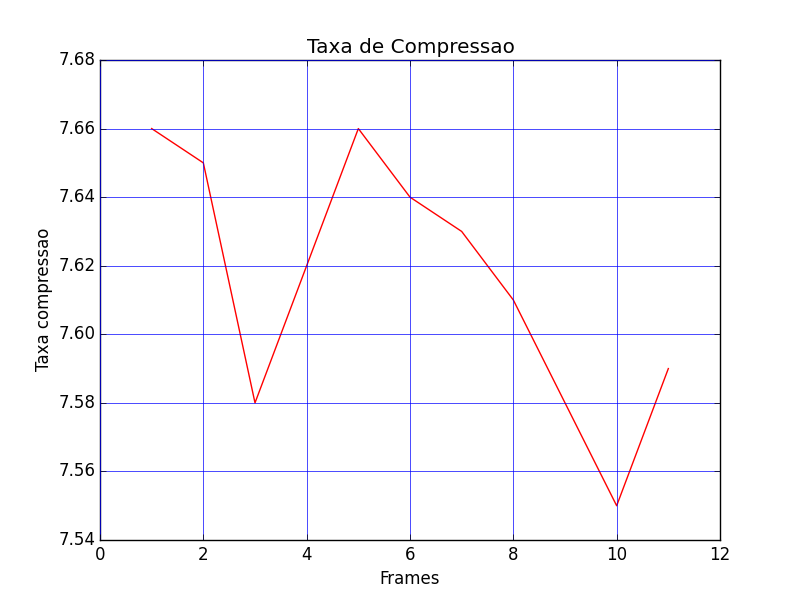
\includegraphics[width=1.2\textwidth]{imagens/ex1_Taxas.png}
        \caption{Taxas de Compressão.}
    \end{minipage}\hfill
    \begin{minipage}{0.45\textwidth}
        \centering
        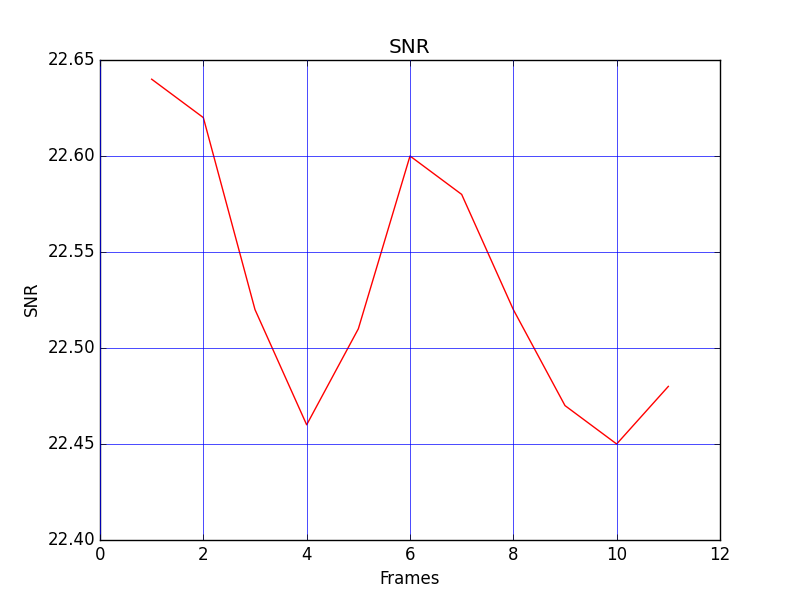
\includegraphics[width=1.2\textwidth]{imagens/ex1_SNR.png}
        \caption{Relação Sinal-Ruído}
    \end{minipage}
\end{figure}
%------------------------------------------------------
\begin{figure}[h]
	\centering
    \begin{minipage}{0.45\textwidth}
        \centering
        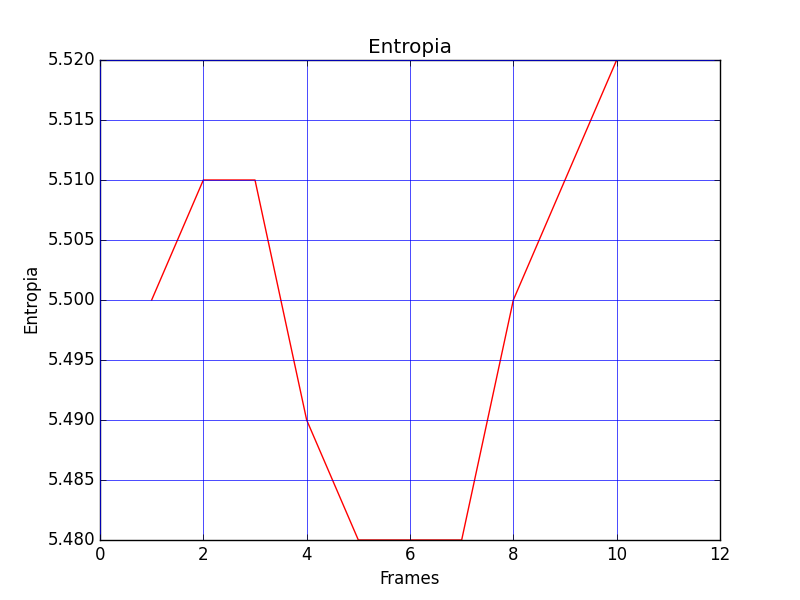
\includegraphics[width=1.2\textwidth]{imagens/ex1_Entropia.png}
        \caption{Entropia.}
    \end{minipage}\hfill
    \begin{minipage}{0.45\textwidth}
        \centering
        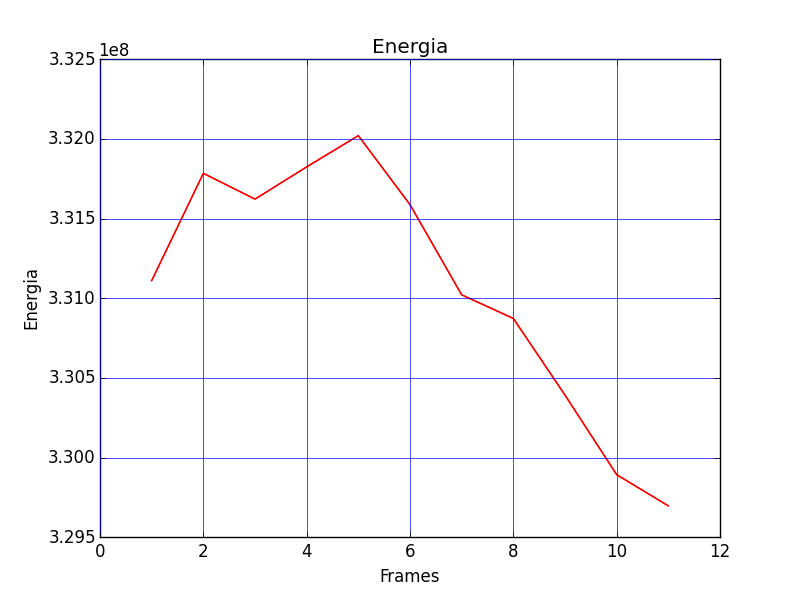
\includegraphics[width=1.2\textwidth]{imagens/ex1_Energia.png}
        \caption{Energia média por píxel.}
    \end{minipage}
\end{figure}
\newpage
\subsection{Codificação inter-frame sem compensação de Movimento}
O segundo método de codificação, tem como objetivo, a codificação das frames de vídeo considerando estas como inter-frames (P), à exceção da primeira, que é uma intra-frame (I). Neste modo, é realizada a codificação da intra-frame (I) do mesmo modo que se realizou no capitulo anterior, de seguida, cada frame (P) é codificada realizando a diferença entre a intra-frame (I) e a P frame atual, finalmente é realizada a codificação da diferença, sem compensação de movimento. No que diz respeito ao descodificador, o processo realizado é o inverso do codificador.

É possível observar nas Figuras 7, 8 e 9 os resultados obtidos na codificação e na descodificação. 

\begin{figure}[h]
	\centering
    \begin{minipage}{0.45\textwidth}
        \centering
        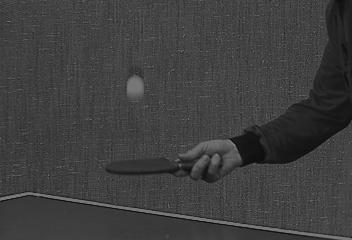
\includegraphics[width=0.8\textwidth]{imagens/bola_1.jpeg}
        \caption{Intra-frame (I).}
    \end{minipage}\hfill
    \begin{minipage}{0.45\textwidth}
        \centering
        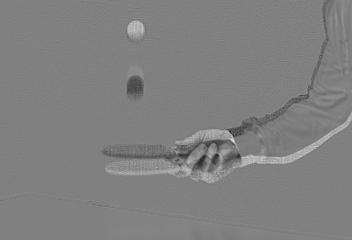
\includegraphics[width=0.8\textwidth]{imagens/bola_8.jpeg}
        \caption{Diferença entre frames.}
    \end{minipage}
    \begin{minipage}{0.45\textwidth}
        \centering
        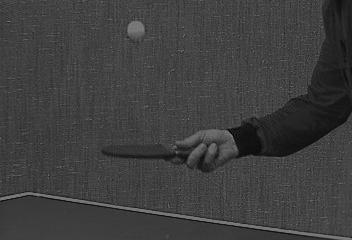
\includegraphics[width=0.8\textwidth]{imagens/bola_88.jpeg}
        \caption{Descodificação da frame 8.}
    \end{minipage}
\end{figure}

A Figura 7 representa a intra-frame (I) à qual foi realizada uma codificação JPEG. A Figura 8 representa a codificação da diferença entre a frame (I) e a frame 8 da sequência de vídeo. Comparando a Figura 7 e 8 é possível observar na Figura 8 que todo o fundo da imagem permaneceu igual, pois não existiu movimento, e apenas a zona da bola e da raquete é que foi codificada. Na Figura 9 temos um exemplo da descodificação da frame 8.
\newpage
Tal como na parte 1 do trabalho foram realizados os cálculos das Taxas de Compressão, Relação Sinal-Ruído, Entropia e Energia média por píxel. É possível observar nas Figuras 10, 11, 12 e 13 os resultados obtidos em comparação com o codificador implementado na parte 1 do trabalho.

\begin{figure}[h]
	\centering
    \begin{minipage}{0.45\textwidth}
        \centering
        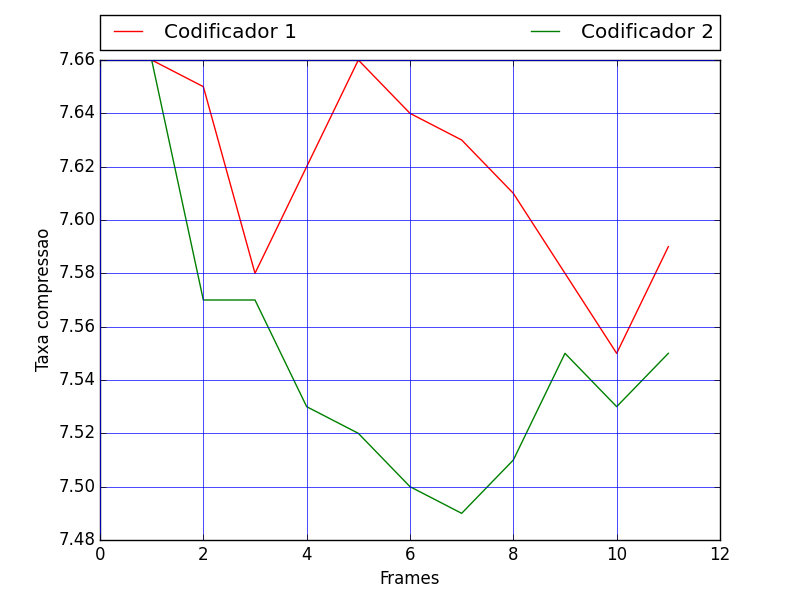
\includegraphics[width=1.2\textwidth]{imagens/Taxas.png}
        \caption{Taxas de Compressão.}
    \end{minipage}\hfill
    \begin{minipage}{0.45\textwidth}
        \centering
        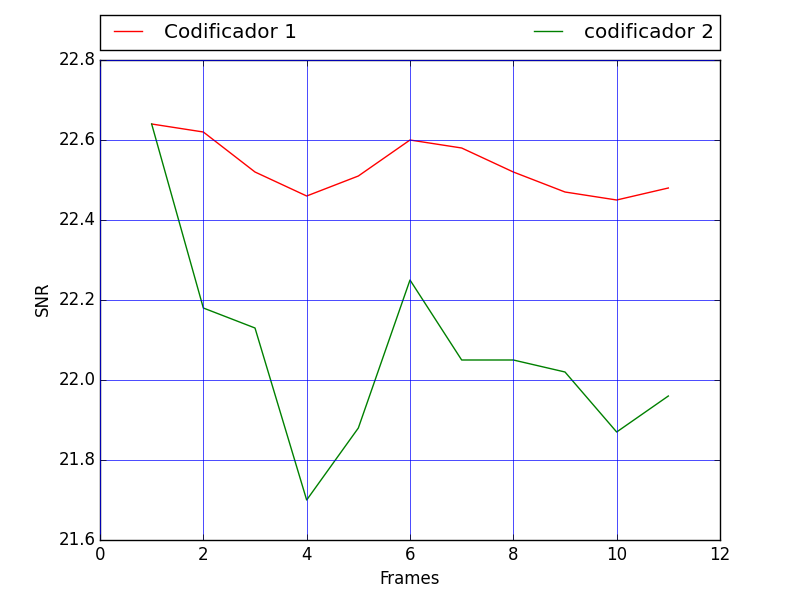
\includegraphics[width=1.2\textwidth]{imagens/SNR.png}
        \caption{Relação Sinal-Ruído.}
    \end{minipage}
\end{figure}
%------------------------------------------------------
\begin{figure}[h]
	\centering
    \begin{minipage}{0.45\textwidth}
        \centering
        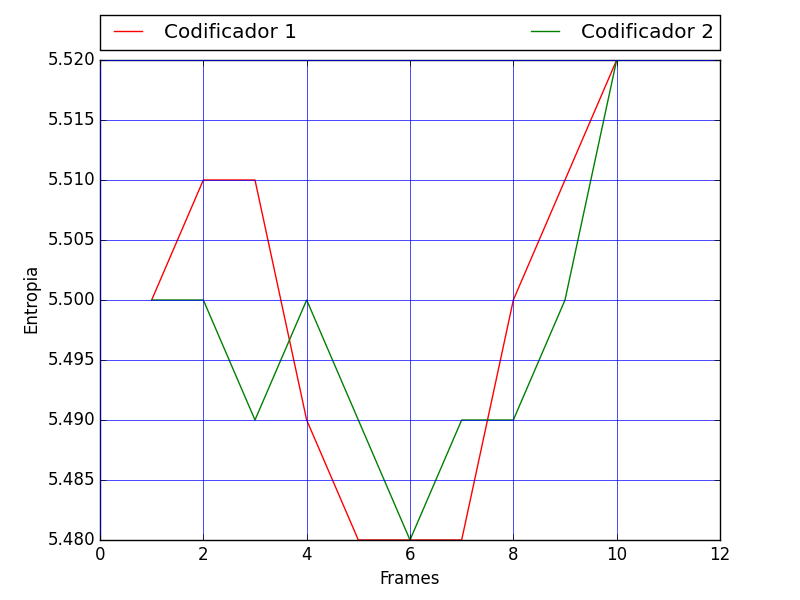
\includegraphics[width=1.2\textwidth]{imagens/Entropia.png}
        \caption{Entropia.}
    \end{minipage}\hfill
    \begin{minipage}{0.45\textwidth}
        \centering
        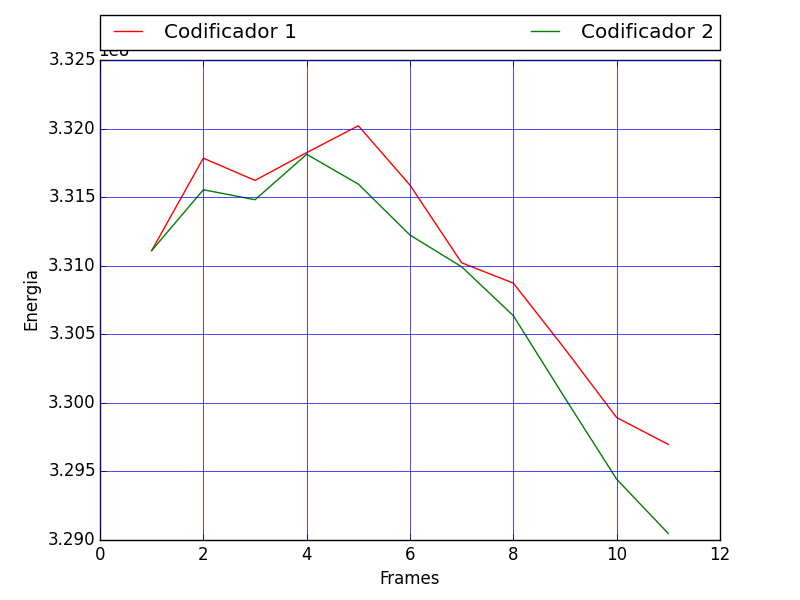
\includegraphics[width=1.2\textwidth]{imagens/Energia.png}
        \caption{Energia média p/ píxel.}
    \end{minipage}
\end{figure}

Observando os resultados obtidos podemos reparar que na Figura 10 existe uma diminuição na Taxa de Compressão no codificador dois, isto significa que são necessários um maior número de bits para representar as imagens utilizando o codificador do segundo ponto do trabalho.

No que diz respeito à Relação Sinal-Ruído apresentada na Figura 11, é possível observar uma ligeira descida da mesma, deste modo, implica uma maior introdução de ruído por parte do codificador 2. 

Tanto a energia média por píxel como a Entropia mantiveram-se significativamente idênticas à exceção de umas ligeiras oscilações.

\subsection{Codificação inter-frame com compensação de movimento}
O terceiro ponto do trabalho prático requer a implementação de uma codificação inter-frame utilizando compensação de movimento. É considerado que cada frame à exceção da primeira é uma inter-frame (P). Ao contrário do ponto anterior a predição da frame a codificar é implementada com base na I-frame utilizando a compensação de movimento. Finalmente, a frame a transmitir é a diferença entre a frame a codificar e a sua predição.

De modo a implementar este codificador foi necessário construir as seguintes funções:
\begin{itemize}
\item Uma função que permita realizar a medição do erro absoluto médio (MAE) entre dois blocos;
\item Uma função que realize a pesquisa do bloco da frame a codificar numa janela de pesquisa (-15 a +15) da frame I-frame;
\item Uma função que percorra os blocos da frame a codificar e construa a frame predita;
\end{itemize}
\newpage
\subsection{Pesquisa full-search}
O tipo de pesquisa implementada no codificador do trabalho foi a pesquisa full-search, para realizar este tipo de pesquisa começámos por selecionar um bloco de 16x16 na janela de procura e medido o erro absoluto médio entre esse bloco e o bloco atual recebido. Caso o valor obtido seja menor que o que foi dados inicialmente como referência, significa que o bloco que estamos a analisar é o mais parecido ao bloco atual. O bloco mais aproximado é então guardado e o valor do erro mínimo absoluto é atualizado.

Após a pesquisa estar concluída obtemos o bloco mais aproximado ao ao bloco P e as coordenadas desse bloco. 

É possível observar na Figura 14 o código desenvolvido que permite a implementação da procura full-search.

\begin{figure}[h]
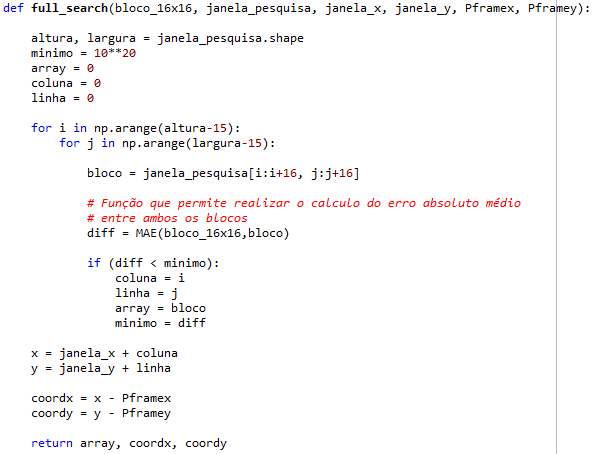
\includegraphics[scale=0.8]{imagens/fullSearch.png}
\centering
\caption{Algoritmo de pesquisa full-search.}
\end{figure}
\newpage
\subsection{Predição de movimento}
De forma a percorrer os blocos da frame a codificar, são selecionados os blocos de 16x16 de forma progressiva na imagem recebida e selecionada também uma janela de pesquisa com dimensão -15 a 15. Após selecionadas ambas as janelas é realizada a pesquisa full-search apresentada na Figura 14.

De modo a selecionar a janela de pesquisa é calculado o valor máximo que o \textit{x} e o \textit{y} podem tomar. Seguidamente, são realizadas as exceções caso o bloco esteja a ocupar a primeira coluna, a primeira linha, a ultima coluna e a ultima linha.

Podemos observar na Figura 15 o algoritmo desenvolvido que permite realizar a predição de movimento.

\begin{figure}[h]
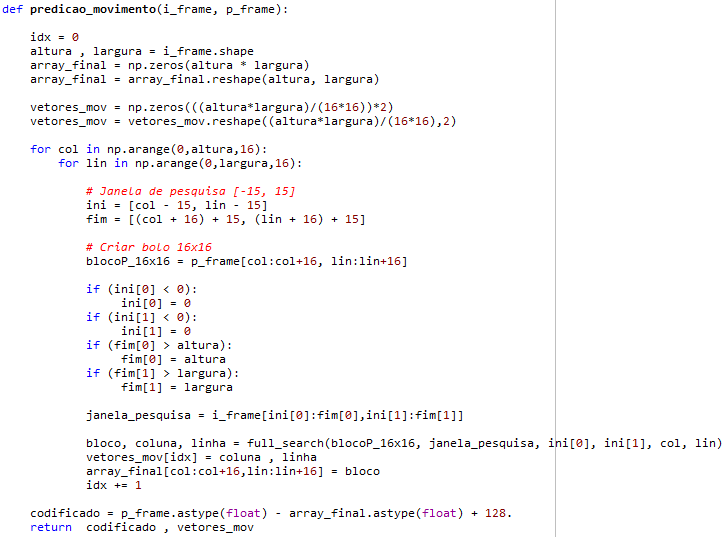
\includegraphics[scale=0.8]{imagens/predicMov.png}
\centering
\caption{Predição de movimento.}
\end{figure}

\subsection{Codificação}
Para a implementação do codificador é necessário fazer a predição de movimento e o método de pesquisa full-search para todas as imagens. O codificador implementado devolve os vetores de movimento que vão ser utilizados posteriormente para realizar a descodificação das frames. Com o codificador desenvolvido é possível observar na Figura 16 a frame 2 resultante da codificação onde é possível observar no "fundo" a frame (I) utilizada para a predição de movimento. 

\begin{figure}[h]
	\centering
    \begin{minipage}{0.4\textwidth}
        \centering
        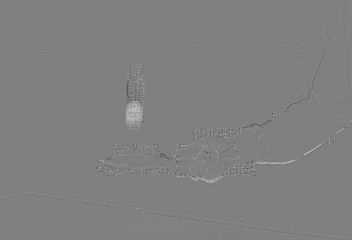
\includegraphics[width=1.2\textwidth]{imagens/bola_2.jpeg}
        \caption{Frame 2 codificada.}
    \end{minipage}\hfill
    \begin{minipage}{0.4\textwidth}
        \centering
        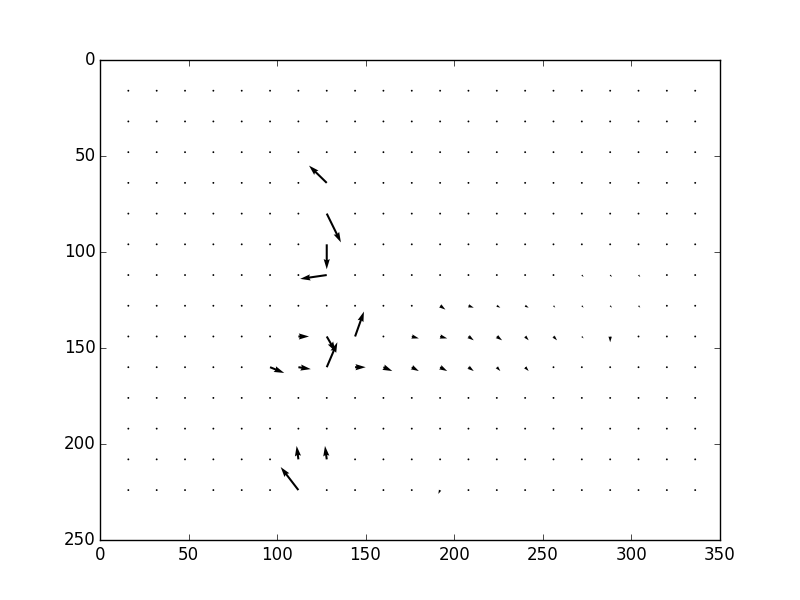
\includegraphics[width=1.2\textwidth]{imagens/1.png}
        \caption{Vetores de movimento.}
    \end{minipage}
\end{figure}
\newpage
\subsection{Descodificação}
Para efetuar a descodificação das imagens e obter as frames originais, foi criada uma função que recebe como argumentos os vetores retornados pela codificação. De seguida, é obtida a frame de referência (I-frame) e são percorridas as outras imagens, onde vamos criar uma matriz de zeros com o tamanho da frame atual e selecionamos o primeiro bloco de 16x16 fazendo-o corresponder a um bloco de 16x16 da frame de referência. Para efetuar essa correspondência utilizamos os vetores de movimento. Caso os vetores de movimento não sejam os dois nulos o bloco desloca-se, caso contrário o bloco é o primeiro e fazemos a correspondência entre os mesmos.

No final a matriz de zeros irá ser totalmente preenchida por blocos da frame de referência e é finalizada a descodificação realizando a soma entre ela e a frame com perdição de movimento e é obtida a imagem original.

É possível observar na Figura 18 a frame 2 descodificada, que resulta do processo de descodificação da Figura 16.

\begin{figure}[h]
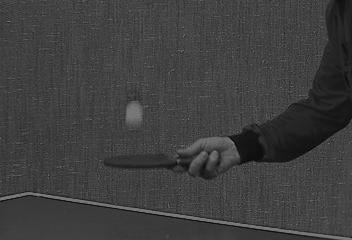
\includegraphics[scale=0.8]{imagens/bola_2_desc.jpeg}
\centering
\caption{Frame 2 descodificada.}
\end{figure}

\newpage

\subsection{Resultados obtidos}
Com a descodificação de todas as frames realizada foram efetuados os cálculos das Taxas de Compressão, Relação Sinal-Ruído, entropia e energia de cada uma. É possível observar nas Figuras seguintes a comparação entre os resultados obtidos nos codificadores 1 e 2 em comparação com o codificador implementado neste ponto.

\begin{figure}[h]
	\centering
    \begin{minipage}{0.45\textwidth}
        \centering
        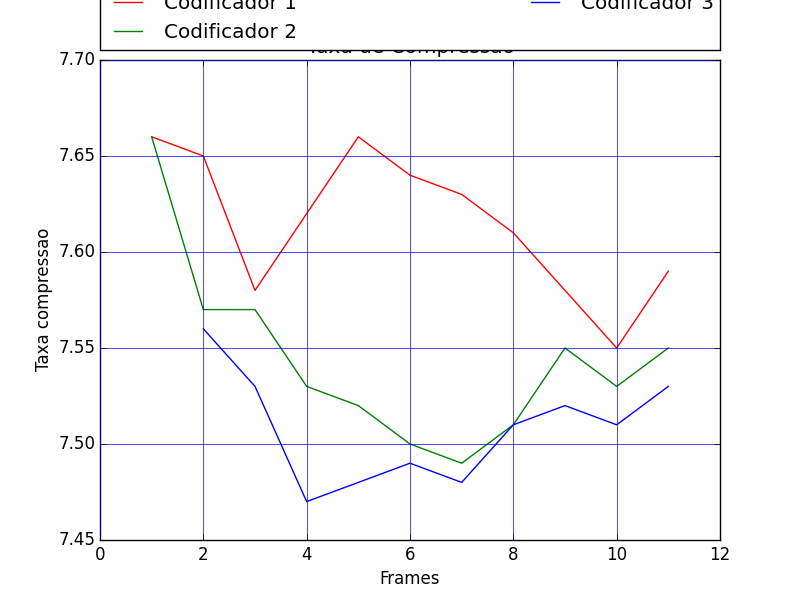
\includegraphics[width=1.2\textwidth]{imagens/Taxas3.png}
        \caption{Taxas de Compressão.}
    \end{minipage}\hfill
    \begin{minipage}{0.45\textwidth}
        \centering
        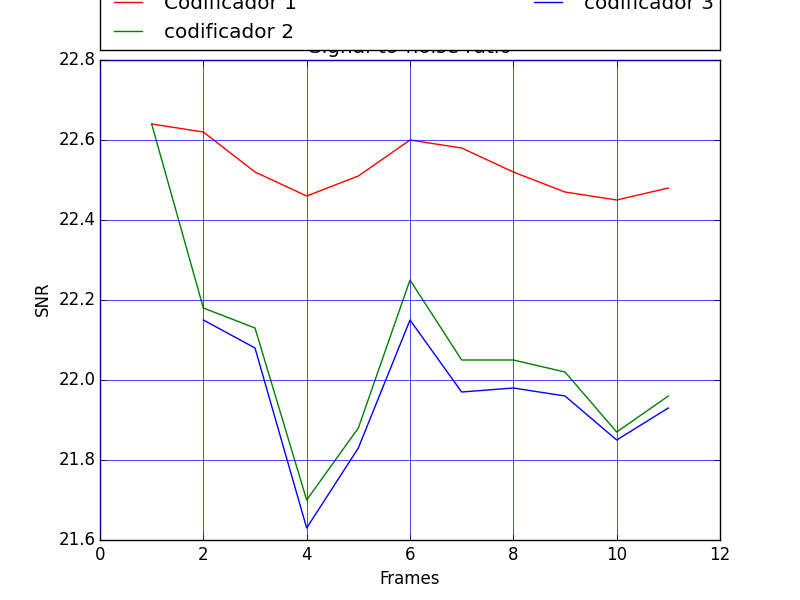
\includegraphics[width=1.2\textwidth]{imagens/SNR3.png}
        \caption{Relação Sinal-Ruído.}
    \end{minipage}
\end{figure}
%------------------------------------------------------
\begin{figure}[h]
	\centering
    \begin{minipage}{0.45\textwidth}
        \centering
        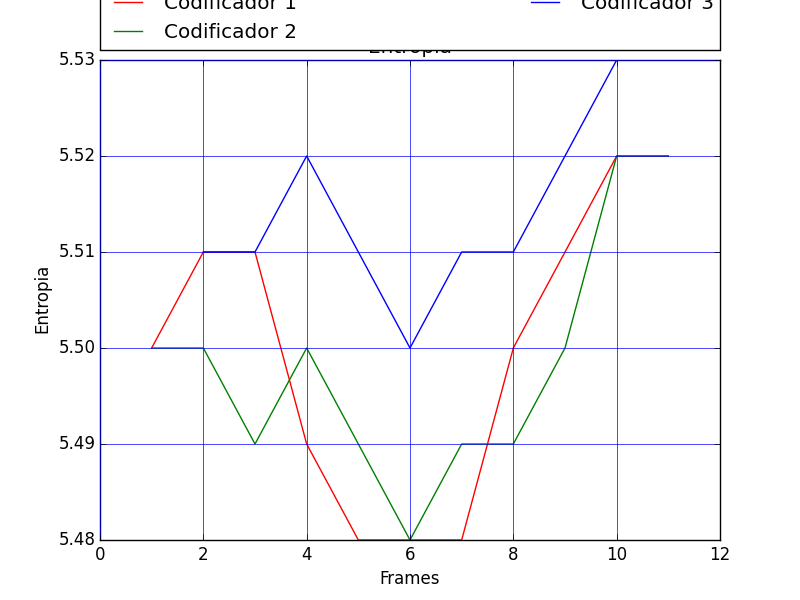
\includegraphics[width=1.2\textwidth]{imagens/Entropia3.png}
        \caption{Entropia.}
    \end{minipage}\hfill
    \begin{minipage}{0.45\textwidth}
        \centering
        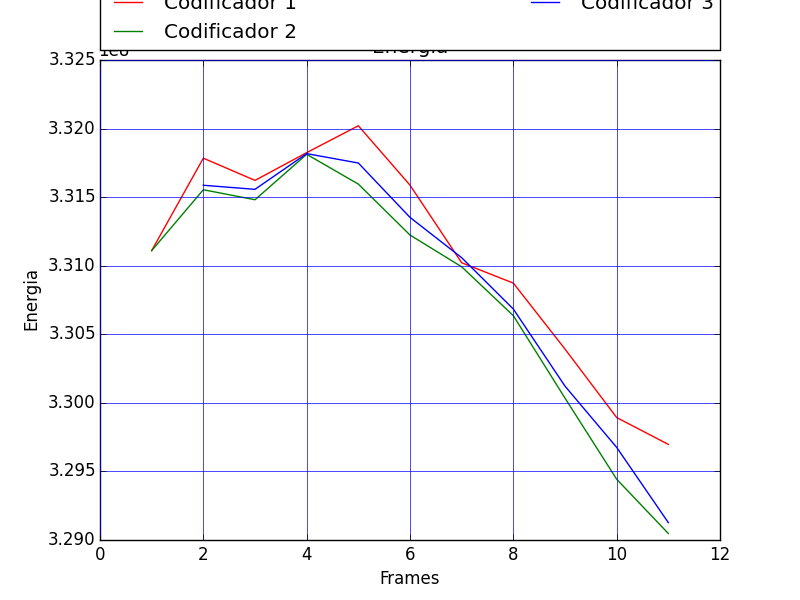
\includegraphics[width=1.2\textwidth]{imagens/Energia3.png}
        \caption{Energia média p/ píxel.}
    \end{minipage}
\end{figure}

É possível observar através dos gráficos apresentados que existiu uma ligeira descida nos valores das Taxas de Compressão em comparação com os codificadores anteriores. A relação Sinal-Ruído manteve-se muito aproximada ao codificador 2, embora tenha existido um aumento na Entropia. Já os valores da energia média por píxel mantiveram-se muito aproximados dos anteriores.

\section{Conclusões}
Observando os resultados obtidos podemos concluir que o trabalho final da disciplina de Codificação de Sinais Multimédia foi desenvolvido com sucesso. Foram implementados todos os pontos existentes no enunciado e os resultados obtidos vão de acordo com o esperado. As imagens resultados da descodificação em todos os pontos são muito aproximadas das imagens originais e é possível observar isso através dos gráficos obtidos. Apenas o codificador do terceiro ponto do trabalho apresenta um tempo de codificação muito elevado pois o processo de codificação com estimação de movimento requer muito processamento. Em suma o grupo encontra-se satisfeito com o desenvolvimento do trabalho.
\end{document}